\documentclass{standalone}
\usepackage{tikz}
\usetikzlibrary{patterns, positioning}

\begin{document}
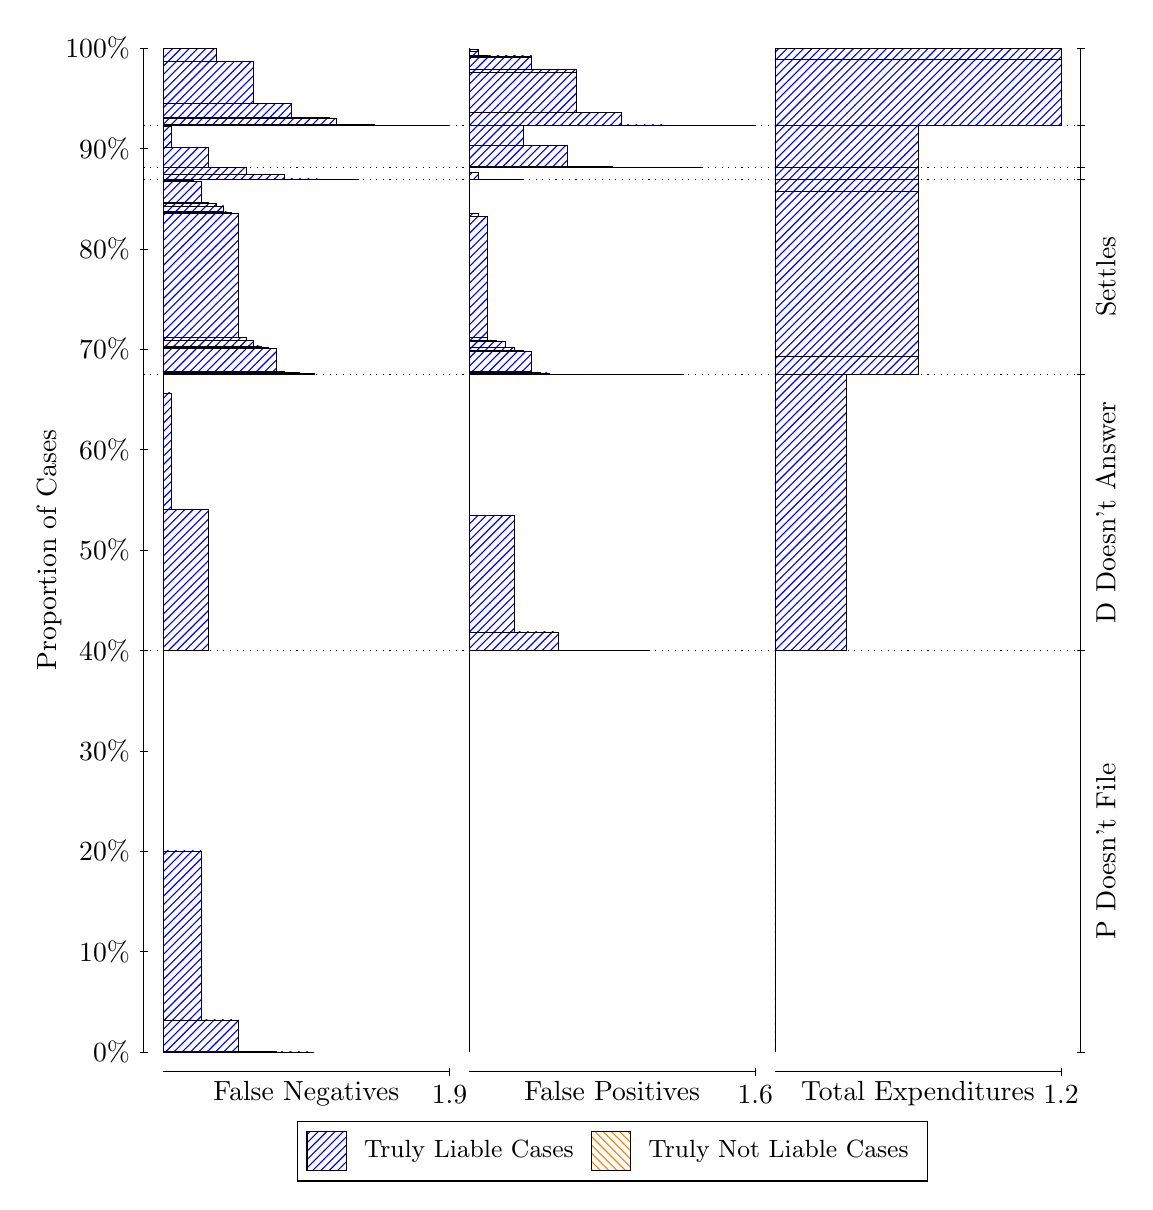
\begin{tikzpicture}
\draw[black, very thin] (1.5,1.75) -- (1.5,14.5);
\node[rotate=90, anchor=center] at (0.3, 8.125) {Proportion of Cases};
\draw[black, very thin] (1.45,1.75) -- (1.55,1.75);
\node[anchor=east] at (1.45, 1.75) {0\%};
\draw[black, very thin] (1.45,3.025) -- (1.55,3.025);
\node[anchor=east] at (1.45, 3.025) {10\%};
\draw[black, very thin] (1.45,4.3) -- (1.55,4.3);
\node[anchor=east] at (1.45, 4.3) {20\%};
\draw[black, very thin] (1.45,5.575) -- (1.55,5.575);
\node[anchor=east] at (1.45, 5.575) {30\%};
\draw[black, very thin] (1.45,6.85) -- (1.55,6.85);
\node[anchor=east] at (1.45, 6.85) {40\%};
\draw[black, very thin] (1.45,8.125) -- (1.55,8.125);
\node[anchor=east] at (1.45, 8.125) {50\%};
\draw[black, very thin] (1.45,9.4) -- (1.55,9.4);
\node[anchor=east] at (1.45, 9.4) {60\%};
\draw[black, very thin] (1.45,10.675) -- (1.55,10.675);
\node[anchor=east] at (1.45, 10.675) {70\%};
\draw[black, very thin] (1.45,11.95) -- (1.55,11.95);
\node[anchor=east] at (1.45, 11.95) {80\%};
\draw[black, very thin] (1.45,13.225) -- (1.55,13.225);
\node[anchor=east] at (1.45, 13.225) {90\%};
\draw[black, very thin] (1.45,14.5) -- (1.55,14.5);
\node[anchor=east] at (1.45, 14.5) {100\%};

\draw[black, very thin] (13.4,1.75) -- (13.4,14.5);
\draw[black, very thin] (13.35,1.75) -- (13.45,1.75);
\node[anchor=west] at (13.35, 1.75) {};
\draw[black, very thin] (13.35,6.8489) -- (13.45,6.8489);
\node[anchor=west] at (13.35, 6.8489) {};
\draw[black, very thin] (13.35,10.356) -- (13.45,10.356);
\node[anchor=west] at (13.35, 10.356) {};
\draw[black, very thin] (13.35,12.834) -- (13.45,12.834);
\node[anchor=west] at (13.35, 12.834) {};
\draw[black, very thin] (13.35,12.986) -- (13.45,12.986);
\node[anchor=west] at (13.35, 12.986) {};
\draw[black, very thin] (13.35,13.516) -- (13.45,13.516);
\node[anchor=west] at (13.35, 13.516) {};
\draw[black, very thin] (13.35,14.5) -- (13.45,14.5);
\node[anchor=west] at (13.35, 14.5) {};

\draw[black, very thin, pattern color=blue, pattern=north east lines] (1.75,1.75) rectangle (3.6623,1.75);
\draw[black, very thin, pattern color=blue, pattern=north east lines] (1.75,1.75) rectangle (3.1842,1.7534);
\draw[black, very thin, pattern color=blue, pattern=north east lines] (1.75,1.7534) rectangle (2.7061,2.158);
\draw[black, very thin, pattern color=blue, pattern=north east lines] (1.75,2.158) rectangle (2.2281,4.3029);
\draw[black, very thin, pattern color=orange, pattern=north west lines] (1.75,4.3029) rectangle (1.75,4.3029);
\draw[black, very thin, pattern color=blue, pattern=north east lines] (1.75,4.3029) rectangle (1.75,6.8489);
\draw[black, very thin, pattern color=blue, pattern=north east lines] (1.75,6.8489) rectangle (2.3237,8.6373);
\draw[black, very thin, pattern color=blue, pattern=north east lines] (1.75,8.6373) rectangle (1.8456,10.121);
\draw[black, very thin, pattern color=orange, pattern=north west lines] (1.75,10.121) rectangle (1.75,10.121);
\draw[black, very thin, pattern color=blue, pattern=north east lines] (1.75,10.121) rectangle (1.75,10.356);
\draw[black, very thin, pattern color=blue, pattern=north east lines] (1.75,10.356) rectangle (3.6623,10.369);
\draw[black, very thin, pattern color=blue, pattern=north east lines] (1.75,10.369) rectangle (3.4711,10.376);
\draw[black, very thin, pattern color=blue, pattern=north east lines] (1.75,10.376) rectangle (3.2798,10.39);
\draw[black, very thin, pattern color=blue, pattern=north east lines] (1.75,10.39) rectangle (3.1842,10.688);
\draw[black, very thin, pattern color=blue, pattern=north east lines] (1.75,10.688) rectangle (3.0886,10.695);
\draw[black, very thin, pattern color=blue, pattern=north east lines] (1.75,10.695) rectangle (2.993,10.718);
\draw[black, very thin, pattern color=blue, pattern=north east lines] (1.75,10.718) rectangle (2.8974,10.787);
\draw[black, very thin, pattern color=blue, pattern=north east lines] (1.75,10.787) rectangle (2.8018,10.829);
\draw[black, very thin, pattern color=blue, pattern=north east lines] (1.75,10.829) rectangle (2.7061,12.398);
\draw[black, very thin, pattern color=blue, pattern=north east lines] (1.75,12.398) rectangle (2.6105,12.42);
\draw[black, very thin, pattern color=blue, pattern=north east lines] (1.75,12.42) rectangle (2.5149,12.427);
\draw[black, very thin, pattern color=blue, pattern=north east lines] (1.75,12.427) rectangle (2.5149,12.496);
\draw[black, very thin, pattern color=blue, pattern=north east lines] (1.75,12.496) rectangle (2.4193,12.531);
\draw[black, very thin, pattern color=blue, pattern=north east lines] (1.75,12.531) rectangle (2.3237,12.544);
\draw[black, very thin, pattern color=blue, pattern=north east lines] (1.75,12.544) rectangle (2.2281,12.808);
\draw[black, very thin, pattern color=blue, pattern=north east lines] (1.75,12.808) rectangle (2.1325,12.815);
\draw[black, very thin, pattern color=blue, pattern=north east lines] (1.75,12.815) rectangle (2.0368,12.815);
\draw[black, very thin, pattern color=blue, pattern=north east lines] (1.75,12.815) rectangle (2.0368,12.832);
\draw[black, very thin, pattern color=blue, pattern=north east lines] (1.75,12.832) rectangle (1.9412,12.833);
\draw[black, very thin, pattern color=blue, pattern=north east lines] (1.75,12.833) rectangle (1.8456,12.833);
\draw[black, very thin, pattern color=orange, pattern=north west lines] (1.75,12.833) rectangle (1.75,12.833);
\draw[black, very thin, pattern color=blue, pattern=north east lines] (1.75,12.833) rectangle (1.75,12.834);
\draw[black, very thin, pattern color=blue, pattern=north east lines] (1.75,12.834) rectangle (4.236,12.834);
\draw[black, very thin, pattern color=blue, pattern=north east lines] (1.75,12.834) rectangle (3.7579,12.838);
\draw[black, very thin, pattern color=blue, pattern=north east lines] (1.75,12.838) rectangle (3.2798,12.895);
\draw[black, very thin, pattern color=blue, pattern=north east lines] (1.75,12.895) rectangle (2.8018,12.984);
\draw[black, very thin, pattern color=blue, pattern=north east lines] (1.75,12.984) rectangle (2.3237,12.986);
\draw[black, very thin, pattern color=orange, pattern=north west lines] (1.75,12.986) rectangle (1.75,12.986);
\draw[black, very thin, pattern color=blue, pattern=north east lines] (1.75,12.986) rectangle (2.3237,13.24);
\draw[black, very thin, pattern color=blue, pattern=north east lines] (1.75,13.24) rectangle (1.8456,13.504);
\draw[black, very thin, pattern color=orange, pattern=north west lines] (1.75,13.504) rectangle (1.75,13.504);
\draw[black, very thin, pattern color=blue, pattern=north east lines] (1.75,13.504) rectangle (1.75,13.516);
\draw[black, very thin, pattern color=blue, pattern=north east lines] (1.75,13.516) rectangle (5.3833,13.516);
\draw[black, very thin, pattern color=blue, pattern=north east lines] (1.75,13.516) rectangle (4.9053,13.517);
\draw[black, very thin, pattern color=blue, pattern=north east lines] (1.75,13.517) rectangle (4.4272,13.535);
\draw[black, very thin, pattern color=blue, pattern=north east lines] (1.75,13.535) rectangle (4.3316,13.535);
\draw[black, very thin, pattern color=blue, pattern=north east lines] (1.75,13.535) rectangle (3.9491,13.611);
\draw[black, very thin, pattern color=blue, pattern=north east lines] (1.75,13.611) rectangle (3.8535,13.616);
\draw[black, very thin, pattern color=blue, pattern=north east lines] (1.75,13.616) rectangle (3.4711,13.618);
\draw[black, very thin, pattern color=blue, pattern=north east lines] (1.75,13.618) rectangle (3.3754,13.792);
\draw[black, very thin, pattern color=blue, pattern=north east lines] (1.75,13.792) rectangle (2.993,13.792);
\draw[black, very thin, pattern color=blue, pattern=north east lines] (1.75,13.792) rectangle (2.8974,14.331);
\draw[black, very thin, pattern color=blue, pattern=north east lines] (1.75,14.331) rectangle (2.5149,14.331);
\draw[black, very thin, pattern color=blue, pattern=north east lines] (1.75,14.331) rectangle (2.4193,14.492);
\draw[black, very thin, pattern color=blue, pattern=north east lines] (1.75,14.492) rectangle (1.9412,14.5);
\draw[black, very thin, pattern color=orange, pattern=north west lines] (1.75,14.5) rectangle (1.75,14.5);
\draw[black, very thin, pattern color=blue, pattern=north east lines] (1.75,14.5) rectangle (1.75,14.5);
\draw[black, very thin, pattern color=orange, pattern=north west lines] (5.6333,1.75) rectangle (5.6333,1.75);
\draw[black, very thin, pattern color=blue, pattern=north east lines] (5.6333,1.75) rectangle (5.6333,6.8489);
\draw[black, very thin, pattern color=orange, pattern=north west lines] (5.6333,6.8489) rectangle (7.9042,6.8489);
\draw[black, very thin, pattern color=blue, pattern=north east lines] (5.6333,6.8489) rectangle (7.9042,6.8489);
\draw[black, very thin, pattern color=blue, pattern=north east lines] (5.6333,6.8489) rectangle (7.3365,6.8492);
\draw[black, very thin, pattern color=blue, pattern=north east lines] (5.6333,6.8492) rectangle (6.7687,7.084);
\draw[black, very thin, pattern color=blue, pattern=north east lines] (5.6333,7.084) rectangle (6.201,8.5673);
\draw[black, very thin, pattern color=blue, pattern=north east lines] (5.6333,8.5673) rectangle (5.6333,10.356);
\draw[black, very thin, pattern color=orange, pattern=north west lines] (5.6333,10.356) rectangle (8.3583,10.356);
\draw[black, very thin, pattern color=blue, pattern=north east lines] (5.6333,10.356) rectangle (8.3583,10.356);
\draw[black, very thin, pattern color=orange, pattern=north west lines] (5.6333,10.356) rectangle (8.1313,10.356);
\draw[black, very thin, pattern color=blue, pattern=north east lines] (5.6333,10.356) rectangle (8.1313,10.356);
\draw[black, very thin, pattern color=orange, pattern=north west lines] (5.6333,10.356) rectangle (7.9042,10.356);
\draw[black, very thin, pattern color=blue, pattern=north east lines] (5.6333,10.356) rectangle (7.9042,10.356);
\draw[black, very thin, pattern color=blue, pattern=north east lines] (5.6333,10.356) rectangle (7.7906,10.356);
\draw[black, very thin, pattern color=orange, pattern=north west lines] (5.6333,10.356) rectangle (7.6771,10.356);
\draw[black, very thin, pattern color=blue, pattern=north east lines] (5.6333,10.356) rectangle (7.6771,10.356);
\draw[black, very thin, pattern color=blue, pattern=north east lines] (5.6333,10.356) rectangle (7.5635,10.356);
\draw[black, very thin, pattern color=orange, pattern=north west lines] (5.6333,10.356) rectangle (7.45,10.356);
\draw[black, very thin, pattern color=blue, pattern=north east lines] (5.6333,10.356) rectangle (7.45,10.356);
\draw[black, very thin, pattern color=blue, pattern=north east lines] (5.6333,10.356) rectangle (7.3365,10.356);
\draw[black, very thin, pattern color=orange, pattern=north west lines] (5.6333,10.356) rectangle (7.2229,10.356);
\draw[black, very thin, pattern color=blue, pattern=north east lines] (5.6333,10.356) rectangle (7.2229,10.356);
\draw[black, very thin, pattern color=blue, pattern=north east lines] (5.6333,10.356) rectangle (7.1094,10.356);
\draw[black, very thin, pattern color=blue, pattern=north east lines] (5.6333,10.356) rectangle (6.9958,10.357);
\draw[black, very thin, pattern color=orange, pattern=north west lines] (5.6333,10.357) rectangle (6.9958,10.357);
\draw[black, very thin, pattern color=blue, pattern=north east lines] (5.6333,10.357) rectangle (6.9958,10.357);
\draw[black, very thin, pattern color=blue, pattern=north east lines] (5.6333,10.357) rectangle (6.8823,10.357);
\draw[black, very thin, pattern color=blue, pattern=north east lines] (5.6333,10.357) rectangle (6.7687,10.358);
\draw[black, very thin, pattern color=blue, pattern=north east lines] (5.6333,10.358) rectangle (6.6552,10.375);
\draw[black, very thin, pattern color=blue, pattern=north east lines] (5.6333,10.375) rectangle (6.5417,10.382);
\draw[black, very thin, pattern color=blue, pattern=north east lines] (5.6333,10.382) rectangle (6.4281,10.401);
\draw[black, very thin, pattern color=blue, pattern=north east lines] (5.6333,10.401) rectangle (6.4281,10.646);
\draw[black, very thin, pattern color=blue, pattern=north east lines] (5.6333,10.646) rectangle (6.3146,10.659);
\draw[black, very thin, pattern color=blue, pattern=north east lines] (5.6333,10.659) rectangle (6.201,10.694);
\draw[black, very thin, pattern color=blue, pattern=north east lines] (5.6333,10.694) rectangle (6.0875,10.77);
\draw[black, very thin, pattern color=blue, pattern=north east lines] (5.6333,10.77) rectangle (5.974,10.792);
\draw[black, very thin, pattern color=blue, pattern=north east lines] (5.6333,10.792) rectangle (5.8604,10.827);
\draw[black, very thin, pattern color=blue, pattern=north east lines] (5.6333,10.827) rectangle (5.8604,12.361);
\draw[black, very thin, pattern color=blue, pattern=north east lines] (5.6333,12.361) rectangle (5.7469,12.403);
\draw[black, very thin, pattern color=blue, pattern=north east lines] (5.6333,12.403) rectangle (5.6333,12.834);
\draw[black, very thin, pattern color=orange, pattern=north west lines] (5.6333,12.834) rectangle (6.3146,12.834);
\draw[black, very thin, pattern color=blue, pattern=north east lines] (5.6333,12.834) rectangle (6.3146,12.836);
\draw[black, very thin, pattern color=blue, pattern=north east lines] (5.6333,12.836) rectangle (5.7469,12.925);
\draw[black, very thin, pattern color=blue, pattern=north east lines] (5.6333,12.925) rectangle (5.6333,12.986);
\draw[black, very thin, pattern color=orange, pattern=north west lines] (5.6333,12.986) rectangle (8.5854,12.986);
\draw[black, very thin, pattern color=blue, pattern=north east lines] (5.6333,12.986) rectangle (8.5854,12.986);
\draw[black, very thin, pattern color=blue, pattern=north east lines] (5.6333,12.986) rectangle (8.0177,12.986);
\draw[black, very thin, pattern color=blue, pattern=north east lines] (5.6333,12.986) rectangle (7.45,12.998);
\draw[black, very thin, pattern color=blue, pattern=north east lines] (5.6333,12.998) rectangle (6.8823,13.262);
\draw[black, very thin, pattern color=blue, pattern=north east lines] (5.6333,13.262) rectangle (6.3146,13.516);
\draw[black, very thin, pattern color=orange, pattern=north west lines] (5.6333,13.516) rectangle (9.2667,13.516);
\draw[black, very thin, pattern color=blue, pattern=north east lines] (5.6333,13.516) rectangle (9.2667,13.516);
\draw[black, very thin, pattern color=orange, pattern=north west lines] (5.6333,13.516) rectangle (8.699,13.516);
\draw[black, very thin, pattern color=blue, pattern=north east lines] (5.6333,13.516) rectangle (8.699,13.516);
\draw[black, very thin, pattern color=orange, pattern=north west lines] (5.6333,13.516) rectangle (8.1313,13.516);
\draw[black, very thin, pattern color=blue, pattern=north east lines] (5.6333,13.516) rectangle (8.1313,13.524);
\draw[black, very thin, pattern color=blue, pattern=north east lines] (5.6333,13.524) rectangle (7.5635,13.685);
\draw[black, very thin, pattern color=orange, pattern=north west lines] (5.6333,13.685) rectangle (7.5635,13.685);
\draw[black, very thin, pattern color=blue, pattern=north east lines] (5.6333,13.685) rectangle (7.5635,13.685);
\draw[black, very thin, pattern color=orange, pattern=north west lines] (5.6333,13.685) rectangle (7.45,13.685);
\draw[black, very thin, pattern color=blue, pattern=north east lines] (5.6333,13.685) rectangle (7.45,13.685);
\draw[black, very thin, pattern color=blue, pattern=north east lines] (5.6333,13.685) rectangle (6.9958,14.189);
\draw[black, very thin, pattern color=blue, pattern=north east lines] (5.6333,14.189) rectangle (6.9958,14.224);
\draw[black, very thin, pattern color=orange, pattern=north west lines] (5.6333,14.224) rectangle (6.8823,14.224);
\draw[black, very thin, pattern color=blue, pattern=north east lines] (5.6333,14.224) rectangle (6.8823,14.224);
\draw[black, very thin, pattern color=blue, pattern=north east lines] (5.6333,14.224) rectangle (6.4281,14.384);
\draw[black, very thin, pattern color=blue, pattern=north east lines] (5.6333,14.384) rectangle (6.4281,14.399);
\draw[black, very thin, pattern color=blue, pattern=north east lines] (5.6333,14.399) rectangle (6.3146,14.4);
\draw[black, very thin, pattern color=orange, pattern=north west lines] (5.6333,14.4) rectangle (6.3146,14.4);
\draw[black, very thin, pattern color=blue, pattern=north east lines] (5.6333,14.4) rectangle (6.3146,14.401);
\draw[black, very thin, pattern color=blue, pattern=north east lines] (5.6333,14.401) rectangle (5.8604,14.405);
\draw[black, very thin, pattern color=blue, pattern=north east lines] (5.6333,14.405) rectangle (5.8604,14.405);
\draw[black, very thin, pattern color=blue, pattern=north east lines] (5.6333,14.405) rectangle (5.7469,14.465);
\draw[black, very thin, pattern color=blue, pattern=north east lines] (5.6333,14.465) rectangle (5.7469,14.481);
\draw[black, very thin, pattern color=blue, pattern=north east lines] (5.6333,14.481) rectangle (5.6333,14.5);
\draw[black, very thin, pattern color=orange, pattern=north west lines] (9.5167,1.75) rectangle (9.5167,1.75);
\draw[black, very thin, pattern color=blue, pattern=north east lines] (9.5167,1.75) rectangle (9.5167,6.8489);
\draw[black, very thin, pattern color=orange, pattern=north west lines] (9.5167,6.8489) rectangle (10.425,6.8489);
\draw[black, very thin, pattern color=blue, pattern=north east lines] (9.5167,6.8489) rectangle (10.425,10.356);
\draw[black, very thin, pattern color=orange, pattern=north west lines] (9.5167,10.356) rectangle (11.333,10.356);
\draw[black, very thin, pattern color=blue, pattern=north east lines] (9.5167,10.356) rectangle (11.333,10.584);
\draw[black, very thin, pattern color=orange, pattern=north west lines] (9.5167,10.584) rectangle (11.333,10.584);
\draw[black, very thin, pattern color=blue, pattern=north east lines] (9.5167,10.584) rectangle (11.333,12.675);
\draw[black, very thin, pattern color=orange, pattern=north west lines] (9.5167,12.675) rectangle (11.333,12.675);
\draw[black, very thin, pattern color=blue, pattern=north east lines] (9.5167,12.675) rectangle (11.333,12.834);
\draw[black, very thin, pattern color=orange, pattern=north west lines] (9.5167,12.834) rectangle (11.333,12.834);
\draw[black, very thin, pattern color=blue, pattern=north east lines] (9.5167,12.834) rectangle (11.333,12.986);
\draw[black, very thin, pattern color=orange, pattern=north west lines] (9.5167,12.986) rectangle (11.333,12.986);
\draw[black, very thin, pattern color=blue, pattern=north east lines] (9.5167,12.986) rectangle (11.333,13.516);
\draw[black, very thin, pattern color=orange, pattern=north west lines] (9.5167,13.516) rectangle (13.15,13.516);
\draw[black, very thin, pattern color=blue, pattern=north east lines] (9.5167,13.516) rectangle (13.15,14.352);
\draw[black, very thin, pattern color=orange, pattern=north west lines] (9.5167,14.352) rectangle (13.15,14.352);
\draw[black, very thin, pattern color=blue, pattern=north east lines] (9.5167,14.352) rectangle (13.15,14.5);
\draw[black, dotted] (1.5,6.8489) -- (13.4,6.8489);
\draw[black, dotted] (1.5,10.356) -- (13.4,10.356);
\draw[black, dotted] (1.5,12.834) -- (13.4,12.834);
\draw[black, dotted] (1.5,12.986) -- (13.4,12.986);
\draw[black, dotted] (1.5,13.516) -- (13.4,13.516);
\draw[black, very thin] (1.75,1.5) -- (5.3833,1.5);
\node[anchor=north] at (3.5667, 1.5) {False Negatives};
\draw[black, very thin] (5.3833,1.45) -- (5.3833,1.55);
\node[anchor=north] at (5.3833, 1.45) {1.9};

\draw[black, very thin] (5.6333,1.5) -- (9.2667,1.5);
\node[anchor=north] at (7.45, 1.5) {False Positives};
\draw[black, very thin] (9.2667,1.45) -- (9.2667,1.55);
\node[anchor=north] at (9.2667, 1.45) {1.6};

\draw[black, very thin] (9.5167,1.5) -- (13.15,1.5);
\node[anchor=north] at (11.333, 1.5) {Total Expenditures};
\draw[black, very thin] (13.15,1.45) -- (13.15,1.55);
\node[anchor=north] at (13.15, 1.45) {1.2};

\node[black, centered, rotate=90] at (13.72, 4.2994) {P Doesn't File};
\node[black, centered, rotate=90] at (13.72, 8.6023) {D Doesn't Answer};
\node[black, centered, rotate=90] at (13.72, 11.595) {Settles};




\draw (7.449999999999999,1.5) node[draw=none] (baseCoordinate) {};
\begin{scope}[align=center]
        \matrix[scale=0.5, draw=black, below=0.5cm of baseCoordinate, nodes={draw}, column sep=0.1cm]{
            \node[rectangle, draw, minimum width=0.5cm, minimum height=0.5cm, pattern=north east lines, pattern color=blue] {}; &
            \node[draw=none, font=\small] (B) {Truly Liable Cases}; &
            \node[rectangle, draw, minimum width=0.5cm, minimum height=0.5cm, pattern=north west lines, pattern color=orange] {}; &
            \node[draw=none, font=\small] (B) {Truly Not Liable Cases}; \\
            };
\end{scope}

\end{tikzpicture}
\end{document}